% This must be in the first 5 lines to tell arXiv to use pdfLaTeX, which is strongly recommended.
\pdfoutput=1
% In particular, the hyperref package requires pdfLaTeX in order to break URLs across lines.

\documentclass[11pt]{article}
\usepackage{graphicx}

\usepackage{float}

% Remove the "review" option to generate the final version.
% \usepackage[review]{acl}
\usepackage{acl}

% Standard package includes
\usepackage{times}
\usepackage{latexsym}

% For proper rendering and hyphenation of words containing Latin characters (including in bib files)
\usepackage[T1]{fontenc}
% For Vietnamese characters
% \usepackage[T5]{fontenc}
% See https://www.latex-project.org/help/documentation/encguide.pdf for other character sets

% This assumes your files are encoded as UTF8
\usepackage[utf8]{inputenc}

% This is not strictly necessary, and may be commented out,
% but it will improve the layout of the manuscript,
% and will typically save some space.
\usepackage{microtype}

% This is also not strictly necessary, and may be commented out.
% However, it will improve the aesthetics of text in
% the typewriter font.
\usepackage{inconsolata}

% INCLUDE additional packages here:
\usepackage{booktabs}

\usepackage{xcolor}
\newcommand{\todo}[1]{\textcolor{orange}{[TODO: #1]}}

% If the title and author information does not fit in the area allocated, uncomment the following
%
%\setlength\titlebox{<dim>}
%
% and set <dim> to something 5cm or larger.
\title{Bridging Feature Spaces: Survey on Multimodal Large Language Model

% Author information can be set in various styles:
% For several authors from the same institution:
% \author{Author 1 \and ... \and Author n \\
%         Address line \\ ... \\ Address line}
% if the names do not fit well on one line use
%         Author 1 \\ {\bf Author 2} \\ ... \\ {\bf Author n} \\
% For authors from different institutions:
% \author{Author 1 \\ Address line \\  ... \\ Address line
%         \And  ... \And
%         Author n \\ Address line \\ ... \\ Address line}
% To start a seperate ``row'' of authors use \AND, as in
% \author{Author 1 \\ Address line \\  ... \\ Address line
%         \AND
%         Author 2 \\ Address line \\ ... \\ Address line \And
%         Author 3 \\ Address line \\ ... \\ Address line}


 \vspace{1em}
  \small{\normalfont WashU CSE527A Survey Paper} }
  
\author{Jianhong Tu \\
  Washington University in St. Louis \\
  \texttt{jianhong.t@wustl.edu} \\\And
  Second Author \\
  Washington University in St. Louis \\
  \texttt{email@domain} \\\AND
  Third Author \\
  Washington University in St. Louis \\
  \texttt{email@domain} \\}

\begin{document}
\maketitle

\begin{abstract}

\end{abstract}

\section{Introduction}

\subsection{Multimodality}

\subsection{Large Language Model: Deficiencies}

\subsection{Challenges}

\subsection{Tasks and Applications}

\section{Methods}
A multimodal large language model (MLLM) leverages the idea of \textit{natural language supervision} \citep{DBLP:conf/icml/RadfordKHRGASAM21} to enhance the model's awareness of an entity through various input channels by taking advantage of the \textit{emergent capabilities} \citep{DBLP:journals/tmlr/WeiTBRZBYBZMCHVLDF22} of  large language models (LLM), such that a unimodal LLM multi-step can achieve reasoning \citep{DBLP:journals/corr/abs-2112-11446} and instruction following \citep{DBLP:conf/nips/Ouyang0JAWMZASR22}. To limit the scope, this survey focuses on \textbf{Vision-Language Models} (VLM) that accepts textual tokens and images and details the methods to construct a joint feature space for two modalities via step-by-step feature transforming. 

\subsection{Datasets}
Obtaining a large dataset is crucial to the generalization ability of VLM because the quality of unimodal representation learning is positively proportional to the scale of a dataset. Particularly, in learning image representation, the vision transform, a popular choice in VLM architecture, yields a modest accuracy when trained on a mid-sized dataset but performs better than the SOTA ResNet in a set of common image recognition benchmarks when trained on larger datasets \citep{DBLP:conf/iclr/DosovitskiyB0WZ21}. One method to gather sufficient data points is to integrate benchmark datasets across domains. The PaLM-E group, concerning robotic policy in addition to visuals and texts, gathered the image captioning data "COCO", visual question answer data "VQAv2", text corpus "Wikipedia", and robotic navigation data "SayCan" \citet{DBLP:conf/icml/DriessXSLCIWTVY23}. Appendix A summarizes the common datasets. However, crowd-labeled datasets are often limited in size or tailored for tasks other than VLM. There is a trend to exploit the richness of information on the internet by compiling a customized dataset \citep{DBLP:conf/icml/RadfordKHRGASAM21}. \citet{DBLP:conf/iccv/SunMV0S19} utilized YouTube's audio-transcription to gather 176 hours of synchronous video frames and captions through web API, while \citet{DBLP:conf/icml/RadfordKHRGASAM21} collected approximately 400 million pairs of image and descriptions from public sources. 


\subsection{Joint Representation}
LLMs trained on textual data are incompatible with the raw image data as a 3D tensor with height, width, and multiple channels. A common multimodal modeling approach is learning a joint representation of texts, images, and other modalities. Formally, let $X,\; Y$ be the feature spaces, and we intend to find $\phi: X\times Y \rightarrow Z$, where $Z$ is the feature space for the VLM. Due to the cost of training end-to-end multimodel \citep{DBLP:journals/corr/abs-2306-13549}, it is more feasible to concatenate unimodels into a multimodel, where conventional unimodels are pretrained separately. With the LLM as the backbone, the function $\phi$ serves as a learnable interface that projects the image space $X$ onto the embedding space $Z=Y$ \citep{DBLP:journals/corr/abs-2306-13549}, keeping the feature space invariant to pretrained LLMs. 

Pretraining refers to the stage where a task-agnostic model is trained to optimize an objective function in order to capture the general features of data. Akin to pretrained embeddings can capture semantic similarities, pretrained image classifiers can encode abstract signals. Consider a trained deep classifier as a composite function $h \odot \theta$ where $h$ is a SoftMax classifier and $\theta$ is a feature transformation. The function $h$ may be understood as a mapping function from raw feature space to the transformed feature space where the data is linearly separable. \citet{DBLP:conf/iccv/SunMV0S19} obtains such feature mapping by pretraining a ConvNet on the Kinetics dataset then detaching the final SoftMax layer, resulting in 1024-dimensional continuous feature vectors. Continuous features are tokenized using hierarchical K-Means to extract $2^{14}$ centroids as the final image representations. An alternative model is to apply vision transformer, which is an extension of the transformer architecture that conveniently maps images as a sequence of patches into patch embeddings \citep{DBLP:conf/iclr/DosovitskiyB0WZ21, DBLP:conf/icml/DriessXSLCIWTVY23, DBLP:conf/icml/RadfordKHRGASAM21}. However, patch embeddings are not equivalent to the word embeddings. 

\subsection{Multimodal Pretraining}
Unimodal pretraining learns a useful image prior, and multimodal pretraining further establishes the connection between image and word embeddings. Most simply, the connection can be learnt by treating video embeddings as word embeddings. \citet{DBLP:conf/iccv/SunMV0S19} appends the new image embeddings to a pretrained BERT's lookup table and optimizes a weighted sum of unimodel and multimodel objectives detailed in Appendix B. More directly, \textit{contrastive objectives} are used to fine-tune the text and image encoders by explicitly training on a image-caption paring task to maximize the cosine-similarity between paired image and text embeddings. \citep{DBLP:conf/icml/RadfordKHRGASAM21}. Another light-weight training scheme as opposed to the end-to-ending training above, is to learn a linking function that transform images to "prompts" while "freezing" the encoders and the LLM \citep{DBLP:conf/icml/DriessXSLCIWTVY23}. The multimodel is pretrained on a next-sentence prediction tasks with sequence of visual and linguistic embeddings, updating the affine transformation function only.

\subsection{Fine-tuning}
\begin{figure*}[t]
    \centering
    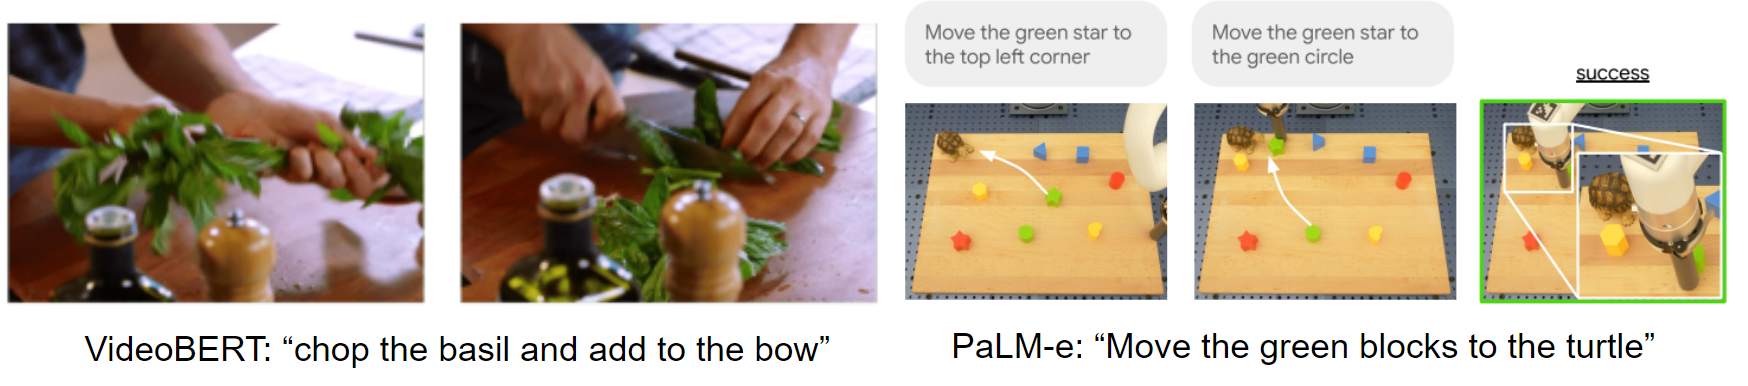
\includegraphics[width=0.80\linewidth]{figures/image.png}
    \caption{Examples of High Level Tasks}
    \label{fig:enter-label}
\end{figure*}
Fine-tuning is a technique to adapt a pretrained model for specific downstream tasks by transferring acquired unimodal knowledge into the final multimodoel. The multimodel optimizes some appropriate objective functions used to assess the model's performance on a curated set of benchmarks, such as visual question answering (VQA) \citep{DBLP:journals/corr/abs-2306-13549}. Fine-tuning enables application of the model in high level tasks, which may be evaluated qualitatively. Figure 2 provides 2 examples: VideoBERT model \citep{DBLP:conf/iccv/SunMV0S19} captions the given image by describing the scene and actions, and predicting successive steps while the PaLM-e model \citep{DBLP:conf/icml/DriessXSLCIWTVY23} generates a robotic policy based on the given prompt.

\section{Results}
Evaluation of multimodels is data and task specific. We generally discusses 3 perspectives to assess model's performance on downstream tasks and the quality of join representation learning.

\subsection{Benchmark scores}
\begin{table}
\scriptsize
\centering
\begin{tabular}{lcccc}
        \toprule
        Model & VQAv2 & & OK-VQA & COCO  \\
        & test-dev & test-std & val & Karpathy test \\
        \midrule
        PaLI-3B & 81.4 & - & 52.4 & 145.4 \\
        PaLI-15B & 82.9 & - & 56.5&  146.2 \\
        PaLI-17B & 84.3 & 84.3 & 64.5 & 149.1\\
        PaLM-E-12B & 77.7 & 77.9 & 60.1 & 136.0 \\
        PaLM-E-66B & - & - & 62.9 & - \\
        PaLM-E-84B & 80.5 & - & 63.3 & 138.0 \\
        \bottomrule
    \end{tabular}
    \caption{Performance of PaLI \citep{DBLP:conf/iclr/Chen0CPPSGGMB0P23} and PaLM-e \citep{DBLP:conf/icml/DriessXSLCIWTVY23} on General Visual-language Benchmarks}
    \label{tab:task_specific_finetuned_models}
\end{table}
Usage of common benchmarks enables cross evaluation of different model. Table 1 provides the reference scores of 2 SOTA MLLM on multimodal tasks. VQA \citep{DBLP:journals/ijcv/GoyalKASBP19} provide image and prompt as the inputs and access the model's ability to retrieve information from the images as the answer to the prompt, while COCO caption \citep{DBLP:journals/corr/ChenFLVGDZ15} let the model to generate context-free description of the image. The scales have a positive impact on both models. 

\subsection{Customized Task Performance}
Models fine-tuned to a more restricted or less common domains tend to assessed using customized benchmarks, and so is their training. VideoBERT \citep{DBLP:conf/iccv/SunMV0S19} is similarly evaluated on video captioning, but on cooking instructional videos. MLLM is also applied to the robotics field with the model as the "brain". PaLM-e \citep{DBLP:conf/icml/DriessXSLCIWTVY23} is able to interact with the environment, which is evaluated on the success rate to carry out human instrcution, i.e. pick up the sponge and then bring it to the user. In a VQA fashion, researchers can assess the model's understanding of the affordance, that whether an \textit{action} can be performed on an \textit{entity}. In addition, \textit{zero-shot classification} is of great interest to understand the generalization, \textit{transfer}, of abstract knowledge into unseen examples. \citet{DBLP:conf/icml/DriessXSLCIWTVY23}, \citet{DBLP:conf/icml/RadfordKHRGASAM21} and \citet{DBLP:conf/iccv/SunMV0S19} report a better zero-shot image classification accuracy than the baseline unimodel and more efficient learning, requiring less data to achieve the same level of performance. 

\subsection{Representation Effectiveness}
Recall that a representation mapping can be obtained by detaching the output layer. The quality of the learnt representation can be thus accessed by the accuracy of a linear classifier on some classification tasks. Compared against ResNet \citep{DBLP:journals/corr/HeZRS15} and BiT-M \citep{DBLP:conf/eccv/KolesnikovBZPYG20}, the features outputted by CLIP \citep{DBLP:conf/iccv/SunMV0S19} achieves a >70\% accuracy on the 16-shot classification tasks versus 63\% and 53\% accuracyf for BiT-M and ResNet respectively, meaning a more effective representation learning result. 

\section{Discussion}

\section{Conclusion}


% Entries for the entire Anthology, followed by custom entries
\bibliography{anthology,custom}
\newpage

\appendix

\section{Example MLLM Datasets}

\begin{table}[H]
    \centering
    \small
    \begin{tabular}{l|l|l|l|}
        \hline
        Dataset & Task & Size \\
        \hline
        TAMP & Robotic manipulation planning with VQA & 96000 scenes & Source\\
        Language Table & Robotic manipulation planning & 600000 sequences & \citet{DBLP:conf/icml/DriessXSLCIWTVY23}\\
        Mobile Manipulation & Robotic navigation and manipulation planing with VQA & 2912 sequences of action & \citet{DBLP:conf/icml/DriessXSLCIWTVY23}\\
        VQA2v & Question answering with images and prompts & 1.1M questions with images &\citet{DBLP:journals/ijcv/GoyalKASBP19}\\
        COCO & Image captioning & 123287 images with captions & \citet{DBLP:journals/corr/ChenFLVGDZ15}\\
        OK-VQA & Visual question answering requiring external knowledge & 14031 questions with images &\citet{DBLP:conf/cvpr/MarinoRFM19}\\
        YouCook & Instructional video captioning & 2000 videos with caption & \citet{DBLP:conf/iccv/SunMV0S19}\\
        CLIP benchmark & Image captioning & 400M image-text pairs & \citet{DBLP:conf/icml/RadfordKHRGASAM21}\\
        \hline
    \end{tabular}
    \caption{Summary of MLLP datasets}
    \onecolumn
\end{table}

\twocolumn
\section{Multimodal BERT Objectives}
\label{sec:appendix}
Pretraining of a multimodel is commonly conducted in a step by step fashion: first the encoders of various modalities is trained, then the pretrained models are concatenated into a multimodel and pretrained on visual-linguistic tasks to acquire a general embedding space of visuals and texts. Here we explain the pretraining objectives of VideoBERT \citep{DBLP:conf/iccv/SunMV0S19} as a paradigm of multimodel pretraining. 

VideoBERT is a masked multimodal large language model. With the images summarised into $2^14$ discrete tokens, both word embeddings and image tokens can be accepted as input to the BERT model. For each modality, the sequences of words or video frames are randomly masked so that the model is trained to restore the maksed embeddings. The video-only training objective is analogous to the text-only, or the valina BERT training objective. It helps the model to acquire long-term state dependencies in video frames. Formally, training each modality separately ensures that the model's capability to capture the marginal distribution of image $P(x)$ or text $P(y)$.

The third training objective to establish the joint distribution $P(x,y)$ so that the model understands the interplay of video and texts. To encode image information into sequences of word embeddings, word-based sentences and visual tokens are combined into visual sentences jointed by a special token "[>]".
\begin{verbatim}
    [CLS] orange chicken with [MASK] sauce 
    [>] v01 [MASK] v08 v72 [SEP]
\end{verbatim}
Researchers proposed a \textit{linguistic-visual alignment} task, where the state of the "[cls]" token is used to determine whether the linguistic sequence and the visual sequence are aligned, which is, to some degree, similar to the \textit{next-sentence prediction} task in the vanila BERT model. This objective essentially establishes the connection between two domains. 

After pretraining, the model would learn a joint representation of multi-modalities. Further fine-tuning allows it to be used into various downstream stasks.


\end{document}
